\documentclass[12pt]{article}
\usepackage{baseset}
\usepackage{myproblem}
\usepackage{stackengine}
\DeclareSymbolFont{operators}{OT1}{ntxtlf}{m}{n}
\SetSymbolFont{operators}{bold}{OT1}{ntxtlf}{b}{n}
\usepackage{wasysym}
\newcommand{\RomanNumeralCaps}[1]
{\MakeUppercase{\romannumeral #1}}
\usepackage{tabularx}
\usepackage{enumitem}

\begin{document}
\begin{tabularx}{\textwidth}{Xr}
{\Large \textbf{Астрофиз}} & Взлёт $12.10.2024$ \\
\end{tabularx}
\noindent\rule{\textwidth}{0.4pt}
\section*{Эффект Доплера и закон Хаббла}
\begin{enumerate}
    \item Линия водорода $H_{\alpha}$  в спектре галактики имеет длину волны $7500$~\AA. Найдите расстояние до галактики. Лабораторная длина волны линии $H_{\alpha}$ равна $6563$~\AA.
    \item Смещение линии $H_{\gamma}$ ($4341$~\AA) составляет $5$ ангстрем. Определите скорость движения источника.
    \item Наклон линий солнечного спектра, наблюдаемых в спектре восточного и западного краев Сатурна, указывает на скорость $19.7$ км/с на экваторе. Определить радиус Юпитера, если наблюдаемый на экваторе его период вращения равен $10^h32^m$.
    \item Определите расстояние до Галактики, если она удаляется от нас со скоростью $7000$ км/с.
    \item В галактике, красное смещение линий в спектре которой соответствует скорости $2000$ км/с, вспыхнула сверхновая звезда. Ее яркость в максимуме была равна $14^m$. Определите абсолютную звездную величину и светимость сверхновой.
    \item Спиральная галактика с красным смещением $0.05$ видна на Земле как узкая полоска длиной $3$ угловые минуты. Лучевая скорость краевых областей галактики отличается от лучевой скорости ее центра на $50$ км/с. Оцените массу галактики.
    \item Галактика A имеет красное смещение $0.07$. Галактика B, расположенная на небе в $120$ градусах от галактики A, имеет красное смещение $0.02$. Какое красное смещение будет иметь галактика B для наблюдателя в галактике A? 
    \item На какой длине волны приходит к нам излучение атомов межзвёздного водорода от галактики, удалённой на расстояние $750$ Мпк? (Длина волны неподвижного источника -- $21$ см).
\end{enumerate}
\section*{Двойные звезды}
\begin{enumerate}[resume]
    \item Две звезды солнечной массы вращаются вокруг общего центра масс по круговым орбитам. Промежуток времени между двумя соседними минимумами $30$ дней. Определите длительность минимума, если наблюдатель находится в плоскости орбиты системы.
    \item Затменная переменная состоит из двух звезд с одинаковым блеском $6^m$ и температурами
	поверхности $5~000$~K и $10~000$ K. Чему равен блеск переменной в моменты главного и вторичного минимумов блеска и вне затмений? Считать, что поверхностная яркость звезды одинакова по всему ее диску, а Земля находится точно в плоскости орбит звезд.
    \item На рисунке приведена кривая блеска  затменно-переменной звезды. Определите по графику блеск компонентов двойной системы.

    \begin{figure}[h] 	
        \centering
        \begin{tikzpicture} 
        \begin{axis}[xlabel=время,
        ylabel=звездная величина, 
        grid=major, 
        y dir=reverse, 
        width=8cm, 
        legend pos = south west,
        ymax=3.2]
        \addplot[line width=1pt, black] coordinates {
            (0, 2)
            (1, 2)
            (1.9, 2.4)
            (2.1, 2.4)
            (3, 2)
            %(4, 2)
            (4, 2)
            (4.9, 3.0)
            (5.1, 3.0)
            (6, 2)
            (7, 2)
            (7.9, 2.4)
            (8.1, 2.4)
            (9, 2)
            (10, 2)
            %(12, 2)
            (10.9, 3.0)
            (11.1, 3.0)
            (12, 2)
            (13, 2)
        };
    
        \end{axis}
        \end{tikzpicture} 
    \end{figure}
    \item Система из двух звезд является затменной переменной, а линия водорода $H_{\alpha}$ ($6563$~\AA) каждые $5$ лет сначала раздваивается на $1.0$~\AA~и $0.75$~\AA, а потом вновь сливается воедино. Чему равно расстояние между звездами? Массы звезд? Сколько длятся транзиты? Линия апсид перпендикулярна лучу зрения.
    \item Перед вами график лучевой скорости двойной звезды. Определите массу компактного невидимого компонента, если масса видимого компонента, у которого измеряли лучевую скорость, составляет $0.5 M_{\odot}$. К какому типу объектов может относиться невидимый компонент?
	\begin{figure}[h]
		\center{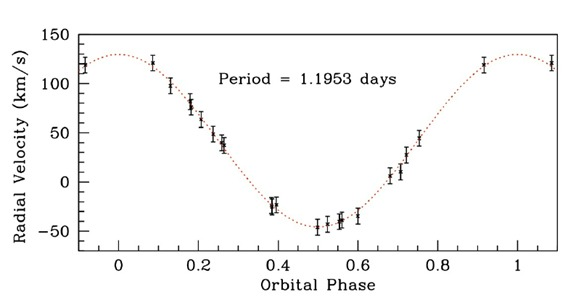
\includegraphics[scale=0.5]{prak3.jpg}}
	\end{figure}
\end{enumerate}
\section*{Законы Талли-Фишера и Фабер-Джексона}
\begin{enumerate}[resume]
    \item Оцените абсолютные звездные величины двух галактик: спиральной со скоростью вращения на палто $150$ км/с и эллиптической с дисперсией скоростей $280$ км/с.
\end{enumerate}
\end{document}